% ---------------------------------------------------------------------------
%  GENERADO AUTOMATICAMENTE por scripts/07_deck_latex.py
%  Las cifras provienen de reports/metrics/*.json. Si reentrenas un modelo,
%  regenera este archivo en vez de editar los numeros a mano:
%      python scripts/07_deck_latex.py
%  (Igual puedes editarlo a mano: es LaTeX normal.)
% ---------------------------------------------------------------------------
\documentclass[aspectratio=169,11pt,table]{beamer}

\usepackage[utf8]{inputenc}
\usepackage[T1]{fontenc}
\usepackage{lmodern}
\usepackage[spanish,es-noshorthands]{babel}
\usepackage{graphicx}
\usepackage{booktabs}
\usepackage{array}
\usepackage{textcomp}
\usepackage{amssymb}

\graphicspath{{figuras/}}

% --- Paleta del proyecto ---------------------------------------------------
\definecolor{verdeosc}{HTML}{2E6B2F}
\definecolor{verdecla}{HTML}{8FB339}
\definecolor{grisTexto}{HTML}{444A52}
\definecolor{grisSuave}{HTML}{8A9098}
\definecolor{grisFondo}{HTML}{F6F7F4}
\definecolor{azul}{HTML}{1F6FB2}
\definecolor{rojo}{HTML}{D1495B}
\definecolor{morado}{HTML}{6A4C93}

% --- Tema ------------------------------------------------------------------
\usetheme{default}
\usefonttheme{professionalfonts}
\setbeamertemplate{navigation symbols}{}
\setbeamercolor{structure}{fg=verdeosc}
\setbeamercolor{normal text}{fg=grisTexto}
\setbeamercolor{frametitle}{fg=verdeosc}
\setbeamercolor{itemize item}{fg=verdecla}
\setbeamercolor{itemize subitem}{fg=verdecla}
\setbeamerfont{frametitle}{size=\Large,series=\bfseries}
\setbeamerfont{framesubtitle}{size=\scriptsize}
\setbeamertemplate{itemize item}{\raisebox{0.15ex}{\tiny$\blacksquare$}}
\setbeamertemplate{itemize subitem}{\raisebox{0.15ex}{\tiny$\square$}}

% Usa \par + \vspace en vez de \\ a proposito: con un subtitulo vacio, un \\
% despues de un grupo vacio provoca "There's no line here to end".
\setbeamertemplate{frametitle}{%
  \vspace*{0.35em}%
  \begin{beamercolorbox}[wd=\paperwidth,leftskip=0.7cm,rightskip=0.7cm]{frametitle}%
    \setlength{\parskip}{0pt}\setlength{\parindent}{0pt}%
    {\usebeamerfont{frametitle}\insertframetitle}\par
    {\usebeamerfont{framesubtitle}\color{grisSuave}\insertframesubtitle}\par
    \vspace{0.2em}%
    {\color{verdecla}\rule{1.7em}{2pt}}%
  \end{beamercolorbox}%
}

\setbeamertemplate{footline}{%
  \hfill{\tiny\color{grisSuave}\insertframenumber\,/\,\inserttotalframenumber}%
  \hspace{0.7cm}\vspace{0.25cm}%
}

% --- Atajos ----------------------------------------------------------------
% Linea de cierre al pie de un slide: el "take-away".
\newcommand{\cierre}[1]{%
  \vfill
  {\color{verdecla}\rule{2.5pt}{0.9em}}\hspace{0.4em}%
  {\footnotesize\color{grisSuave}#1}%
}
% Tarjeta tipo KPI: un numero grande con etiqueta.
\newcommand{\kpi}[4][verdeosc]{%
  \begin{minipage}[t]{#2}%
    \setlength{\fboxsep}{6pt}%
    \colorbox{grisFondo}{\begin{minipage}[t]{\dimexpr\linewidth-2\fboxsep-2\fboxrule\relax}%
      {\tiny\color{grisSuave}\bfseries #3}\\[0.12em]%
      % \large y no \Large: con cinco tarjetas en una fila, un valor como
      % "99,2 %" en \Large desborda la caja.
      {\large\bfseries\color{#1}#4}%
    \end{minipage}}%
  \end{minipage}%
}
% Caja con titulo y borde de color: para contraponer dos ideas lado a lado.
% Se dibuja con LaTeX, no como imagen: una figura hecha de texto queda
% ilegible en cuanto hay que reducirla para que entre en el slide.
\newcommand{\caja}[4][verdeosc]{%
  \begin{minipage}[t]{#2}%
    \setlength{\fboxsep}{7pt}%
    \fcolorbox{#1}{grisFondo}{\begin{minipage}[t]{\dimexpr\linewidth-2\fboxsep-2\fboxrule\relax}%
      {\small\bfseries\color{#1}#3}\\[0.45em]%
      #4%
      \vspace{0.2em}%
    \end{minipage}}%
  \end{minipage}%
}
\newcommand{\sig}{\textcolor{verdeosc}{\textbf{significativa}}}
\newcommand{\nosig}{\textcolor{rojo}{\textbf{NO significativa}}}

\renewcommand{\arraystretch}{1.25}
\setlength{\tabcolsep}{5pt}

% Descomenta para imprimir con notas del orador:
% \setbeameroption{show notes}

\title{Clasificación de madurez de paltas Hass --- Final}
\author{Cristóbal Martínez}

\begin{document}

{
\setbeamercolor{background canvas}{bg=verdeosc}
\begin{frame}[plain]
  \vspace{1.4cm}
  % linespread: a \Huge el interlineado por defecto deja los descendentes de una
  % linea tocando la siguiente.
  {\color{white}\Huge\bfseries\linespread{1.15}\selectfont Clasificación del estado de\\madurez de paltas Hass}

  \vspace{0.55cm}
  {\color{verdecla}\rule{\textwidth}{1.6pt}}

  \vspace{0.55cm}
  {\color{white!85!verdecla}\large ResNet-50, ViT-S/16 e híbridos con presupuesto equiparado}

  \vfill
  {\color{white!70!verdecla}\small Cristóbal Martínez \quad\textbullet\quad Entrega final, 23 de noviembre de 2026}

  \vspace{0.2em}
  {\color{white!60!verdecla}\footnotesize 14.710 fotografías, 478 frutas, índice ordinal de 5 niveles}
  \vspace{0.6cm}
\end{frame}
}

\begin{frame}{El problema}{Por qué importa acá y no solo en el paper}
\begin{columns}[T]
\begin{column}{0.58\textwidth}
{\scriptsize
\setlength{\itemsep}{0.3em}
\begin{itemize}
  \item {\bfseries Chile es uno de los mayores exportadores de palta Hass del mundo.}
  \item La clasificación por madurez se hace hoy a ojo y al tacto, operario por operario, sin criterio homogéneo ni trazabilidad.
  \item Fruta verde en góndola: el consumidor la descarta. Fruta pasada en tránsito: pérdida total. Los dos errores cuestan.
  \item {\bfseries La tarea es \emph{ordinal}, no categórica: $1<2<3<4<5$.}
  \item Confundir un 1 con un 2 es un error de un día. Confundir un 1 con un 5 es mandar fruta podrida a la venta.
\end{itemize}
}
\end{column}
\begin{column}{0.38\textwidth}
{\tiny
\centering
\begin{tabular}{cll}
\toprule
\rowcolor{verdeosc}\color{white}\bfseries Índ. & \color{white}\bfseries Estado & \color{white}\bfseries Decisión \\
\midrule
1 & Verde & Dejar madurar \\
2 & Iniciando & Lista en 2--3 días \\
3 & Maduro I & Venta inmediata \\
4 & Maduro II & Último día \\
5 & Sobremaduro & Fuera de punto \\
\bottomrule
\end{tabular}
}
\end{column}
\end{columns}
\cierre{La métrica tiene que castigar más los errores lejanos. La accuracy plana no lo hace: por eso usamos QWK.}
\end{frame}

\begin{frame}{Datos y limitaciones}{Hass Avocado Ripening Photographic Dataset, Mendeley, CC BY 4.0}
\kpi[verdeosc]{0.224\textwidth}{Imágenes}{14.710}\hfill
\kpi[azul]{0.224\textwidth}{Frutas}{478}\hfill
\kpi[morado]{0.224\textwidth}{Train/val/test}{334/72/72}\hfill
\kpi[rojo]{0.224\textwidth}{Licencia}{CC BY 4.0}
\vspace{0.6em}
{\scriptsize
\setlength{\itemsep}{0.2em}
\begin{itemize}
  \item {\bfseries Que la IA hiciera trampa: resuelto.}
  \item Hay 6.871 pares de fotos casi idénticas de la misma palta en días seguidos. Repartimos las 478 paltas, no las 14.710 fotos, con un chequeo automático que falla si alguna aparece en los dos lados.
  \item {\bfseries El choque con la vida real: no resuelto, declarado.}
  \item Son fotos de laboratorio: fondo blanco, una sola fruta centrada, luz pareja, siempre a la misma distancia. Una foto de celular en una feria no se parece en nada. Es la limitación que decide si esto sirve en una planta empacadora o solo en un informe.
  \item {\bfseries Un solo lote, una sola cosecha, una sola variedad.}
  \item 478 paltas portuguesas de 2022, todas Hass. Y las etiquetas las puso una persona mirando, sin una segunda opinión con qué contrastar: no sabemos cuánto acertaría un experto humano en esta misma tarea.
\end{itemize}
}
\cierre{Detalle completo en la data card (\texttt{entregables/final/data\_card.md}).}
\end{frame}

\begin{frame}{Las dos redes, en una imagen}{La diferencia es CÓMO miran la foto}
\begin{center}
  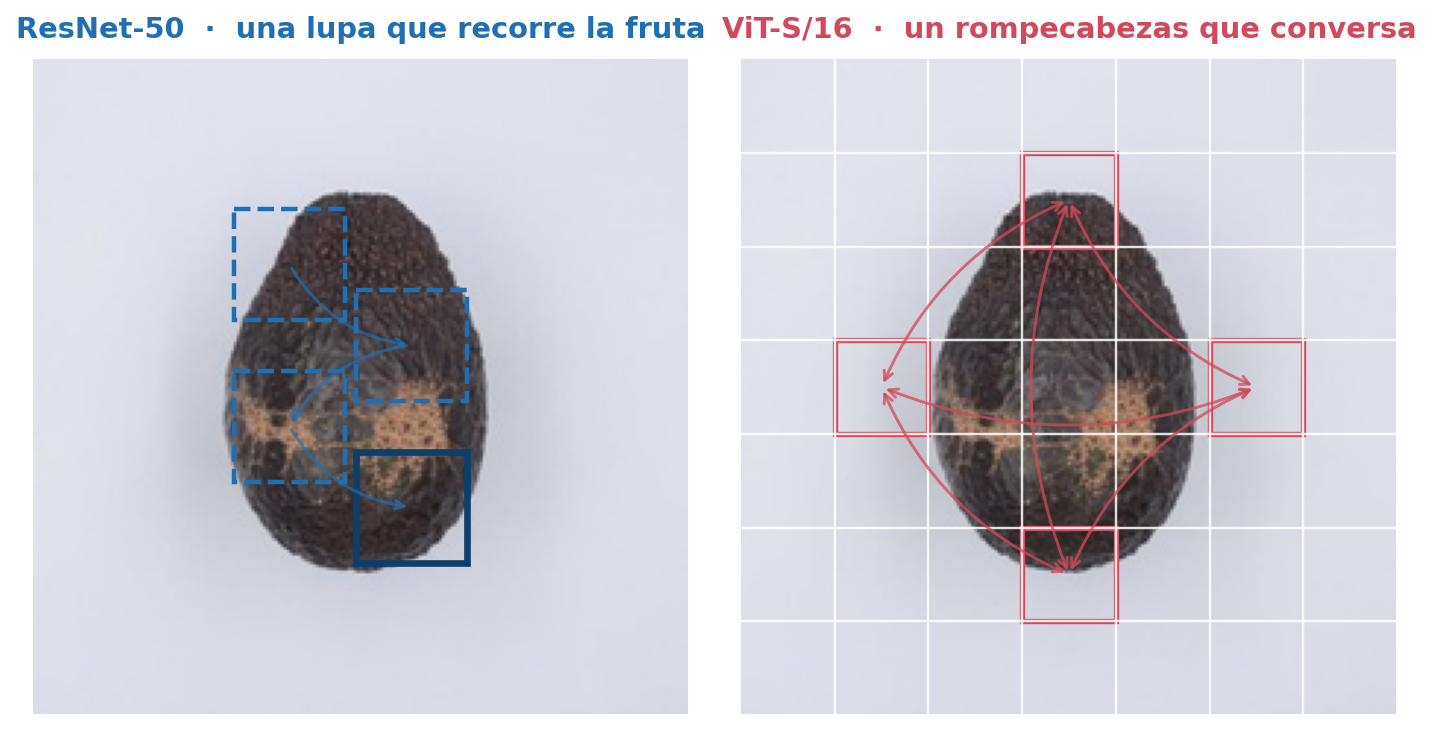
\includegraphics[width=0.95\textwidth,height=4.25cm,keepaspectratio]{30-como-mira-cada-red}
\end{center}
\vspace{0.25em}
\begin{columns}[T]
\begin{column}{0.47\textwidth}
{\tiny
\setlength{\itemsep}{0.12em}
\begin{itemize}
  \item Va de a pedacitos y reutiliza el mismo detector en toda la foto \textit{(convolución)}.
  \item Buena para detalles: manchas, arrugas, tono.
\end{itemize}
}
\end{column}
\begin{column}{0.47\textwidth}
{\tiny
\setlength{\itemsep}{0.12em}
\begin{itemize}
  \item Parte la foto en 196 cuadraditos y los compara todos contra todos \textit{(auto-atención)}.
  \item Buena para relacionar zonas distantes.
\end{itemize}
}
\end{column}
\end{columns}
\cierre{Ninguna se programó desde cero: las dos vienen de \texttt{timm}, la biblioteca estándar de modelos de visión.}
\end{frame}

\begin{frame}{Por qué entrenan tan distinto}{Todo se explica por lo que cada red ya sabe antes de empezar}
\caja[azul]{0.465\textwidth}{ResNet-50 trae dos reglas de fábrica}{{\scriptsize
\setlength{\itemsep}{0.1em}
\begin{itemize}
  \item Lo que importa está \textbf{cerca}
  \item \textbf{No importa} en qué parte de la foto esté
\end{itemize}
}
\vspace{0.25em}
{\tiny\color{grisSuave}\itshape Una mancha café es una mancha café, arriba o abajo de la fruta. Eso no lo aprende: ya lo trae.}}\hfill
\caja[rojo]{0.465\textwidth}{ViT-S/16 no trae ninguna}{{\scriptsize
\setlength{\itemsep}{0.1em}
\begin{itemize}
  \item Todos los cuadraditos le parecen \textbf{iguales}
  \item Ni siquiera sabe cuáles son \textbf{vecinos}
\end{itemize}
}
\vspace{0.25em}
{\tiny\color{grisSuave}\itshape Tiene que deducir de los ejemplos hasta la noción de \guillemotleft{}al lado\guillemotright{}.}}
\vspace{0.55em}
{\tiny
\setlength{\itemsep}{0.2em}
\begin{itemize}
  \item {\bfseries El ViT necesita muchísimos más ejemplos.}
  \item La ResNet arranca sabiendo mirar imágenes; el ViT tiene que descubrir primero \emph{cómo} se mira una imagen, y recién después aprender de paltas.
  \item {\bfseries Por eso los dos parten desde ImageNet.}
  \item Antes de ver una sola palta ya vieron 1,3 millones de fotos de cosas cotidianas. Ahí el ViT compensa: llega con el oficio aprendido.
  \item {\bfseries Y por eso el ViT es más delicado de entrenar.}
  \item Entrenar es bajar un cerro a ciegas y el \emph{learning rate} es el tamaño del paso. La ResNet aguanta pasos grandes; el ViT se cae.
\end{itemize}
}
\end{frame}

\begin{frame}{Los dos híbridos}{Dos formas distintas de juntar ambas ideas}
\begin{columns}[T]
\begin{column}{0.47\textwidth}
{\small\textbf{\color{morado}1. Fusión tardía}}
{\scriptsize
\setlength{\itemsep}{0.15em}
\begin{itemize}
  \item Las dos redes miran la misma foto por separado y al final se juntan sus dos opiniones para decidir.
  \item Como pedir una segunda opinión médica.
  \item Es el único modelo que escribimos nosotros (\texttt{src/paltas/models.py}).
  \item {\bfseries Cuesta el doble: corre las dos redes enteras.}
\end{itemize}
}
\end{column}
\begin{column}{0.47\textwidth}
{\small\textbf{\color{morado}2. ViT-Hybrid R26+S/32}}
{\scriptsize
\setlength{\itemsep}{0.15em}
\begin{itemize}
  \item Una sola red: la parte convolucional procesa la foto primero y le entrega el resultado al transformer.
  \item En vez de dos opiniones, es una cadena de montaje.
  \item Es la arquitectura del paper original de ViT.
  \item {\bfseries Tiene ventaja: más parámetros y más pre-entrenamiento.}
\end{itemize}
}
\end{column}
\end{columns}
\cierre{Ninguno de los dos es equiparable a los baselines, y hay que decirlo: van como referencia, no como competidores.}
\end{frame}

\begin{frame}{Cómo hacemos que la comparación sea justa}{Igualar tres cosas, no solo el tamaño}
{\scriptsize
\centering
\begin{tabular}{lccc}
\toprule
\rowcolor{verdeosc}\color{white}\bfseries Qué igualamos & \color{white}\bfseries ResNet-50 & \color{white}\bfseries ViT-S/16 & \color{white}\bfseries Diferencia \\
\midrule
Tamaño del \guillemotleft{}cerebro\guillemotright{} (conexiones) & 23{,}5 millones & 21{,}7 millones & 7{,}9\,\% \\
Esfuerzo que hace por foto & 8{,}2 mil millones & 8{,}5 mil millones & 3{,}6\,\% \\
Fotos que vio antes de empezar & 1,3 millones & 1,3 millones & ninguna \\
\bottomrule
\end{tabular}
}
\vspace{0.5em}
{\scriptsize
\setlength{\itemsep}{0.25em}
\begin{itemize}
  \item {\bfseries Si una red es más grande y gana, no aprendimos nada: ganó por grande.}
  \item Por eso igualamos el tamaño (parámetros), el trabajo que hace por foto (GFLOPs) y --- lo que casi nadie iguala --- \textbf{cuántas fotos vio antes}.
  \item {\bfseries El tercer punto es el que más distorsiona.}
  \item El ViT que usa todo el mundo viene entrenado con 14 millones de fotos; la ResNet, con 1,3 millones. Comparándolos así estaríamos midiendo quién estudió más, no qué arquitectura es mejor.
  \item Usamos una versión del ViT llamada \textbf{DeiT-S}: es exactamente la misma red, pero entrenada con las mismas 1,3 millones de fotos que la ResNet. Ahí sí la comparación es limpia.
\end{itemize}
}
\cierre{Como comparar dos atletas: sirve si entrenaron lo mismo y compiten en la misma categoría de peso.}
\end{frame}

\begin{frame}{Cómo las entrenamos}{Todo igual para las dos, salvo lo que tiene que cambiar}
\begin{columns}[T]
\begin{column}{0.47\textwidth}
{\small\textbf{Idéntico para ambas}}
{\scriptsize
\setlength{\itemsep}{0.16em}
\begin{itemize}
  \item Las mismas fotos, en el mismo orden
  \item Las mismas deformaciones de las fotos
  \item La misma cantidad de vueltas al dataset
  \item El mismo criterio para elegir el mejor modelo
  \item El mismo criterio para cortar el entrenamiento
\end{itemize}
}
\end{column}
\begin{column}{0.47\textwidth}
{\small\textbf{Distinto en el ViT}}
{\scriptsize\itshape Siguiendo con la imagen del cerro:}
{\scriptsize
\setlength{\itemsep}{0.16em}
\begin{itemize}
  \item {\bfseries Le pedimos pasos 3 veces más cortos.}
  \item Es el \emph{learning rate}. Con pasos largos el ViT tropieza y deja de aprender.
  \item {\bfseries Y que empiece a caminar más lento.}
  \item Es el \emph{warmup}: las primeras vueltas van a media máquina hasta que agarra el ritmo.
\end{itemize}
}
\end{column}
\end{columns}
\vspace{0.4em}
{\scriptsize\textbf{Un detalle que suele hacerse mal:} en casi cualquier otra tarea conviene alterar mucho los colores de las fotos de entrenamiento, para que el modelo no dependa del color. Acá el color \emph{es} la respuesta: si alteramos mucho el tono, una palta clase 2 se vuelve idéntica a una clase 4 pero con la etiqueta vieja. Le estaríamos enseñando mal. Por eso el color casi no se toca; girar y recortar la foto, en cambio, sí.}
\cierre{Igualar el learning rate \guillemotleft{}por justicia\guillemotright{} no sería más justo: sería solo peor para el ViT.}
\end{frame}

{
\setbeamercolor{background canvas}{bg=grisFondo}
\begin{frame}[plain]
  \vfill
  \hspace{0.6cm}{\color{verdecla}\fontsize{54}{58}\selectfont\bfseries 01}%
  \hspace{0.5cm}{\color{verdeosc}\Huge\bfseries Resultados}
  \vfill
\end{frame}
}

\begin{frame}{Todos los modelos, lado a lado}{Medido sobre 2.262 fotos de 72 paltas que ningún modelo había visto}
{\scriptsize
\centering
\begin{tabular}{l >{\centering\arraybackslash}p{0.20\textwidth} >{\centering\arraybackslash}p{0.17\textwidth} c}
\toprule
\rowcolor{verdeosc}\color{white}\bfseries Modelo & \color{white}\bfseries Acierta o se pasa por un escalón & \color{white}\bfseries Error promedio & \color{white}\bfseries Clase exacta \\
\midrule
ResNet-50 & 99{,}2\,\% & 0{,}26 escalones & 74{,}6\,\% \\
ViT-S/16 & 99{,}5\,\% & 0{,}28 escalones & 72{,}2\,\% \\
ResNet-50 (scratch) & 97{,}7\,\% & 0{,}35 escalones & 67{,}2\,\% \\
ViT-S/16 (scratch) & 98{,}1\,\% & 0{,}41 escalones & 61{,}2\,\% \\
Híbrido: fusión tardía & 99{,}5\,\% & 0{,}24 escalones & 76{,}7\,\% \\
\rowcolor{verdecla!22}ViT-Hybrid R26+S/32 & 99{,}6\,\% & 0{,}24 escalones & 76{,}2\,\% \\
\bottomrule
\end{tabular}
}
\vspace{0.6em}
{\scriptsize
\setlength{\itemsep}{0.22em}
\begin{itemize}
  \item {\bfseries Todos los modelos con pre-entrenamiento están sobre el 99\,\%.}
  \item La diferencia entre ellos es de décimas. Los dos que aparecen abajo son los entrenados desde cero, y se nota.
  \item {\bfseries El renglón que importa es el del medio.}
  \item Menos de medio escalón de error promedio significa, en la práctica, medio día de maduración.
\end{itemize}
}
\cierre{La tabla completa, con las seis métricas técnicas, está en el anexo.}
\end{frame}

\begin{frame}{ResNet-50 frente a ViT-S/16}{El resultado central del avance}
\begin{center}
  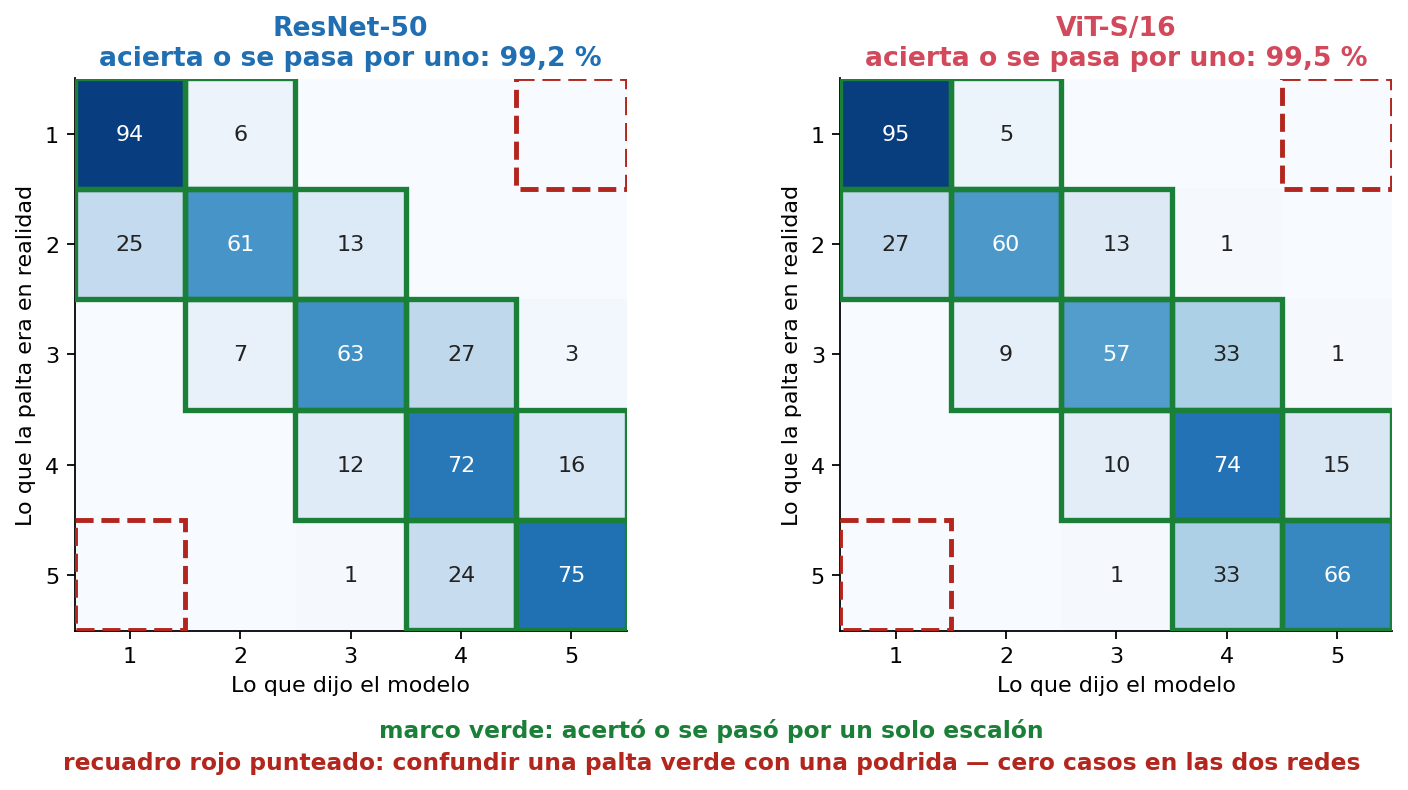
\includegraphics[width=0.86\textwidth,height=3.6cm,keepaspectratio]{33-matrices-didactica}
\end{center}
\vspace{0.3em}
{\tiny
\setlength{\itemsep}{0.2em}
\begin{itemize}
  \item {\bfseries Las dos rinden prácticamente igual.}
  \item La ResNet acierta la clase exacta un poco más seguido. Pero cuando el ViT se equivoca, se equivoca por menos. Se compensa.
  \item Hicimos la prueba estadística formal y la diferencia entre ambas no es concluyente: para efectos prácticos, empatan.
  \item {\bfseries Pero no se equivocan en las mismas fotos.}
  \item Fallan las dos a la vez en solo 18{,}0\,\% de los casos. Si alguien pudiera elegir siempre cuál de las dos tiene razón, acertaría 82{,}0\,\% en vez de 74{,}6\,\%.
  \item Eso es lo que van a intentar aprovechar los modelos híbridos.
\end{itemize}
}
\cierre{Los números completos y las pruebas estadísticas están en el anexo.}
\end{frame}

\begin{frame}{El experimento que lo demuestra}{Reentrenamos las dos redes SIN ImageNet, solo con las fotos de paltas}
\begin{center}
  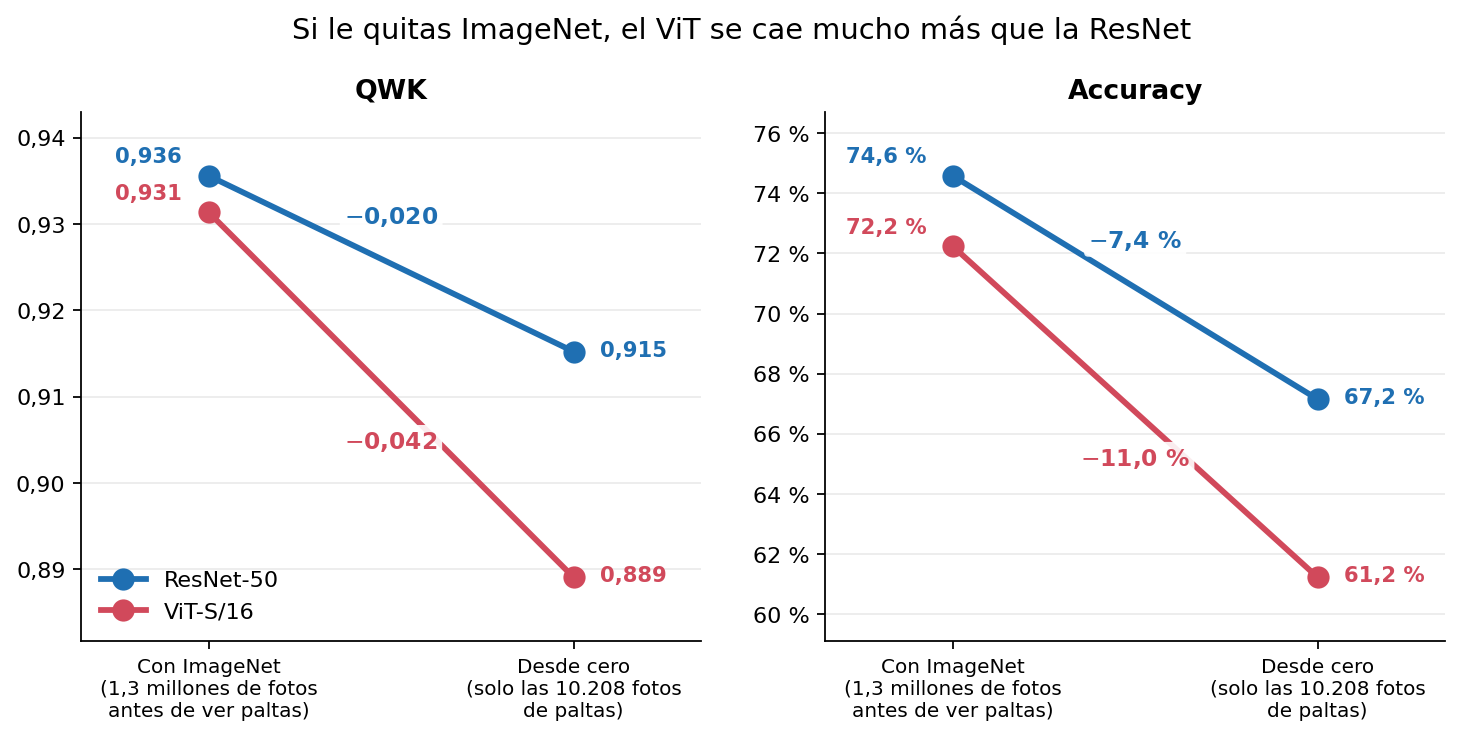
\includegraphics[width=0.84\textwidth,height=3.6cm,keepaspectratio]{32-dependencia-pretraining}
\end{center}
\vspace{0.3em}
{\tiny
\setlength{\itemsep}{0.22em}
\begin{itemize}
  \item {\bfseries El ViT pierde 2{,}1$\times$ más QWK y 1{,}5$\times$ más accuracy que la ResNet.}
  \item Es lo que predice la idea de las \guillemotleft{}reglas de fábrica\guillemotright{}: la ResNet ya sabía mirar imágenes, el ViT tenía que aprenderlo, y 10.208 fotos de paltas no alcanzan para eso.
  \item Las cuatro caídas son estadísticamente sólidas ($p<0{,}0001$), y cada red se compara contra \emph{su propia} versión con ImageNet.
\end{itemize}
}
\cierre{Con ImageNet las dos empatan. Sin ImageNet, no. La diferencia real entre ellas no es el techo, es cuántos datos necesitan para llegar.}
\end{frame}

\begin{frame}{Y hay una segunda razón}{Esta tarea juega en la cancha de la convolución}
{\small
\setlength{\itemsep}{0.3em}
\begin{itemize}
  \item {\bfseries El estado de madurez se lee en detalles pequeños y locales.}
  \item El color de la cáscara, las manchas, el arrugamiento. Todo eso está repartido por la superficie de la fruta y se ve de cerca.
  \item {\bfseries Justo lo que la ResNet hace bien con su lupa.}
  \item La gran ventaja del ViT es relacionar zonas lejanas de una imagen. Acá no hay nada lejano que relacionar: todas las paltas tienen la misma forma, están centradas y sobre el mismo fondo.
  \item {\bfseries Por eso el empate no es casualidad.}
  \item En un problema donde importara la composición global de la escena, probablemente el ViT sacaría ventaja. En este, su superpoder no suma.
\end{itemize}
}
\cierre{Conclusión honesta: no es que el ViT sea peor, es que este problema no le pide lo que él hace mejor.}
\end{frame}

\begin{frame}{Los híbridos}{\textquestiondown{}Suma combinar ambos enfoques?}
\kpi[morado]{0.47\textwidth}{Híbrido: fusión tardía}{QWK 0{,}941}\hfill
\kpi[morado]{0.47\textwidth}{ViT-Hybrid R26+S/32}{QWK 0{,}941}
\vspace{0.3em}
{\scriptsize
\setlength{\itemsep}{0.15em}
\begin{itemize}
  \item Híbrido: fusión tardía: 46{,}4\,M params, 16{,}7 GFLOPs, acc 76{,}7\,\%
  \item ViT-Hybrid R26+S/32: 36{,}0\,M params, 6{,}9 GFLOPs, acc 76{,}2\,\%
\end{itemize}
}
\vspace{0.3em}
\begin{columns}[T]
\begin{column}{0.52\textwidth}
{\tiny
\setlength{\itemsep}{0.22em}
\begin{itemize}
  \item En su tabla de desacuerdo, fusión y ResNet fallan \emph{a la vez} en 20{,}6\,\% de las imágenes: más que el 18{,}0\,\% del par ResNet/ViT. La fusión no elimina los casos difíciles, los absorbe.
  \item {\bfseries La fusión tardía cuesta el doble de cómputo por imagen.}
  \item Dos backbones completos en el forward. La pregunta no es si mejora, sino si mejora lo suficiente para justificar $2\times$ de latencia.
  \item Alcanza su mejor checkpoint en la \textbf{época 2} (3{,}5 min) con los backbones congelados: las representaciones ya contenían la información, lo que faltaba era combinarlas.
\end{itemize}
}
\end{column}
\begin{column}{0.44\textwidth}
\begin{center}
  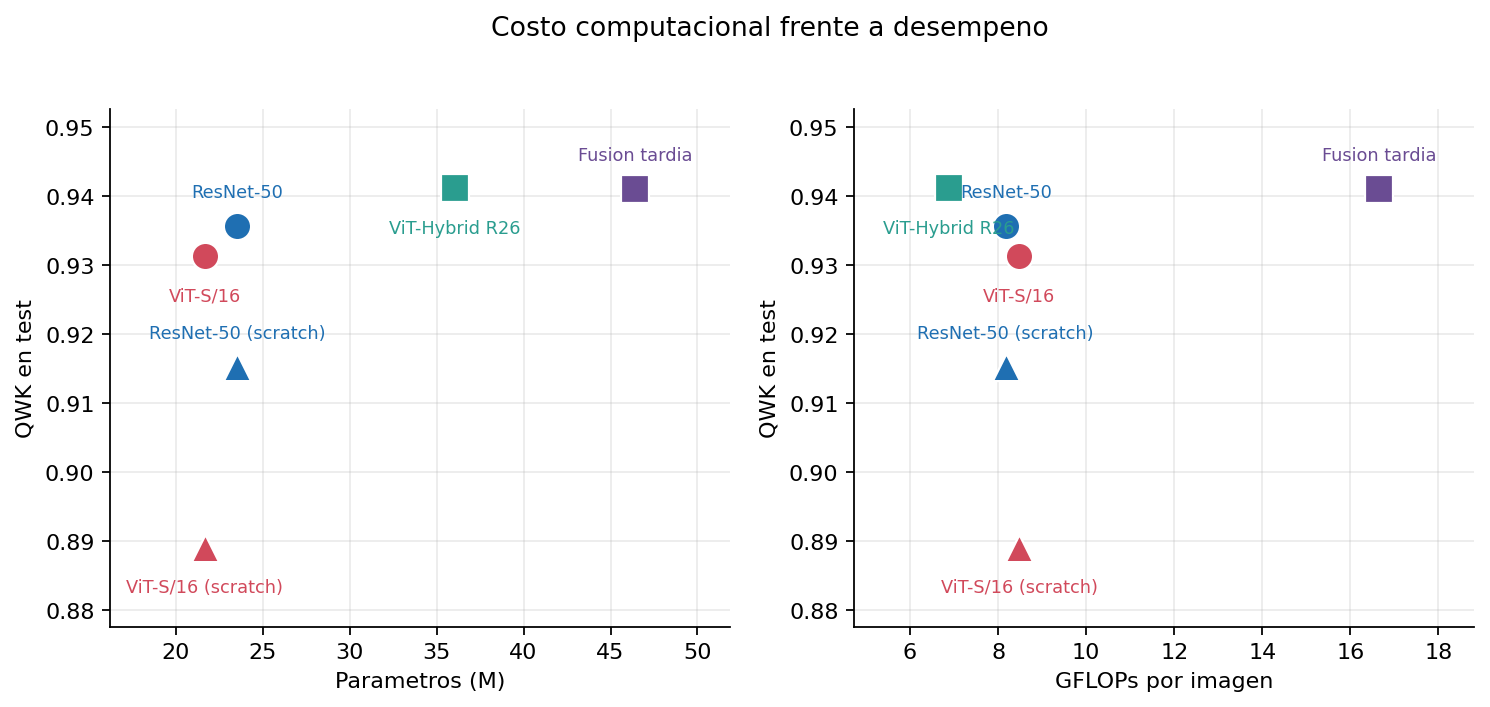
\includegraphics[width=\textwidth,height=2.9cm,keepaspectratio]{13-costo-beneficio-final}
\end{center}
\end{column}
\end{columns}
\end{frame}

\begin{frame}{\textquestiondown{}En qué se fijó el modelo para decidir?}{Pintamos sobre la foto las zonas que más pesaron en la respuesta}
\begin{columns}[T]
\begin{column}{0.30\textwidth}
\begin{center}
  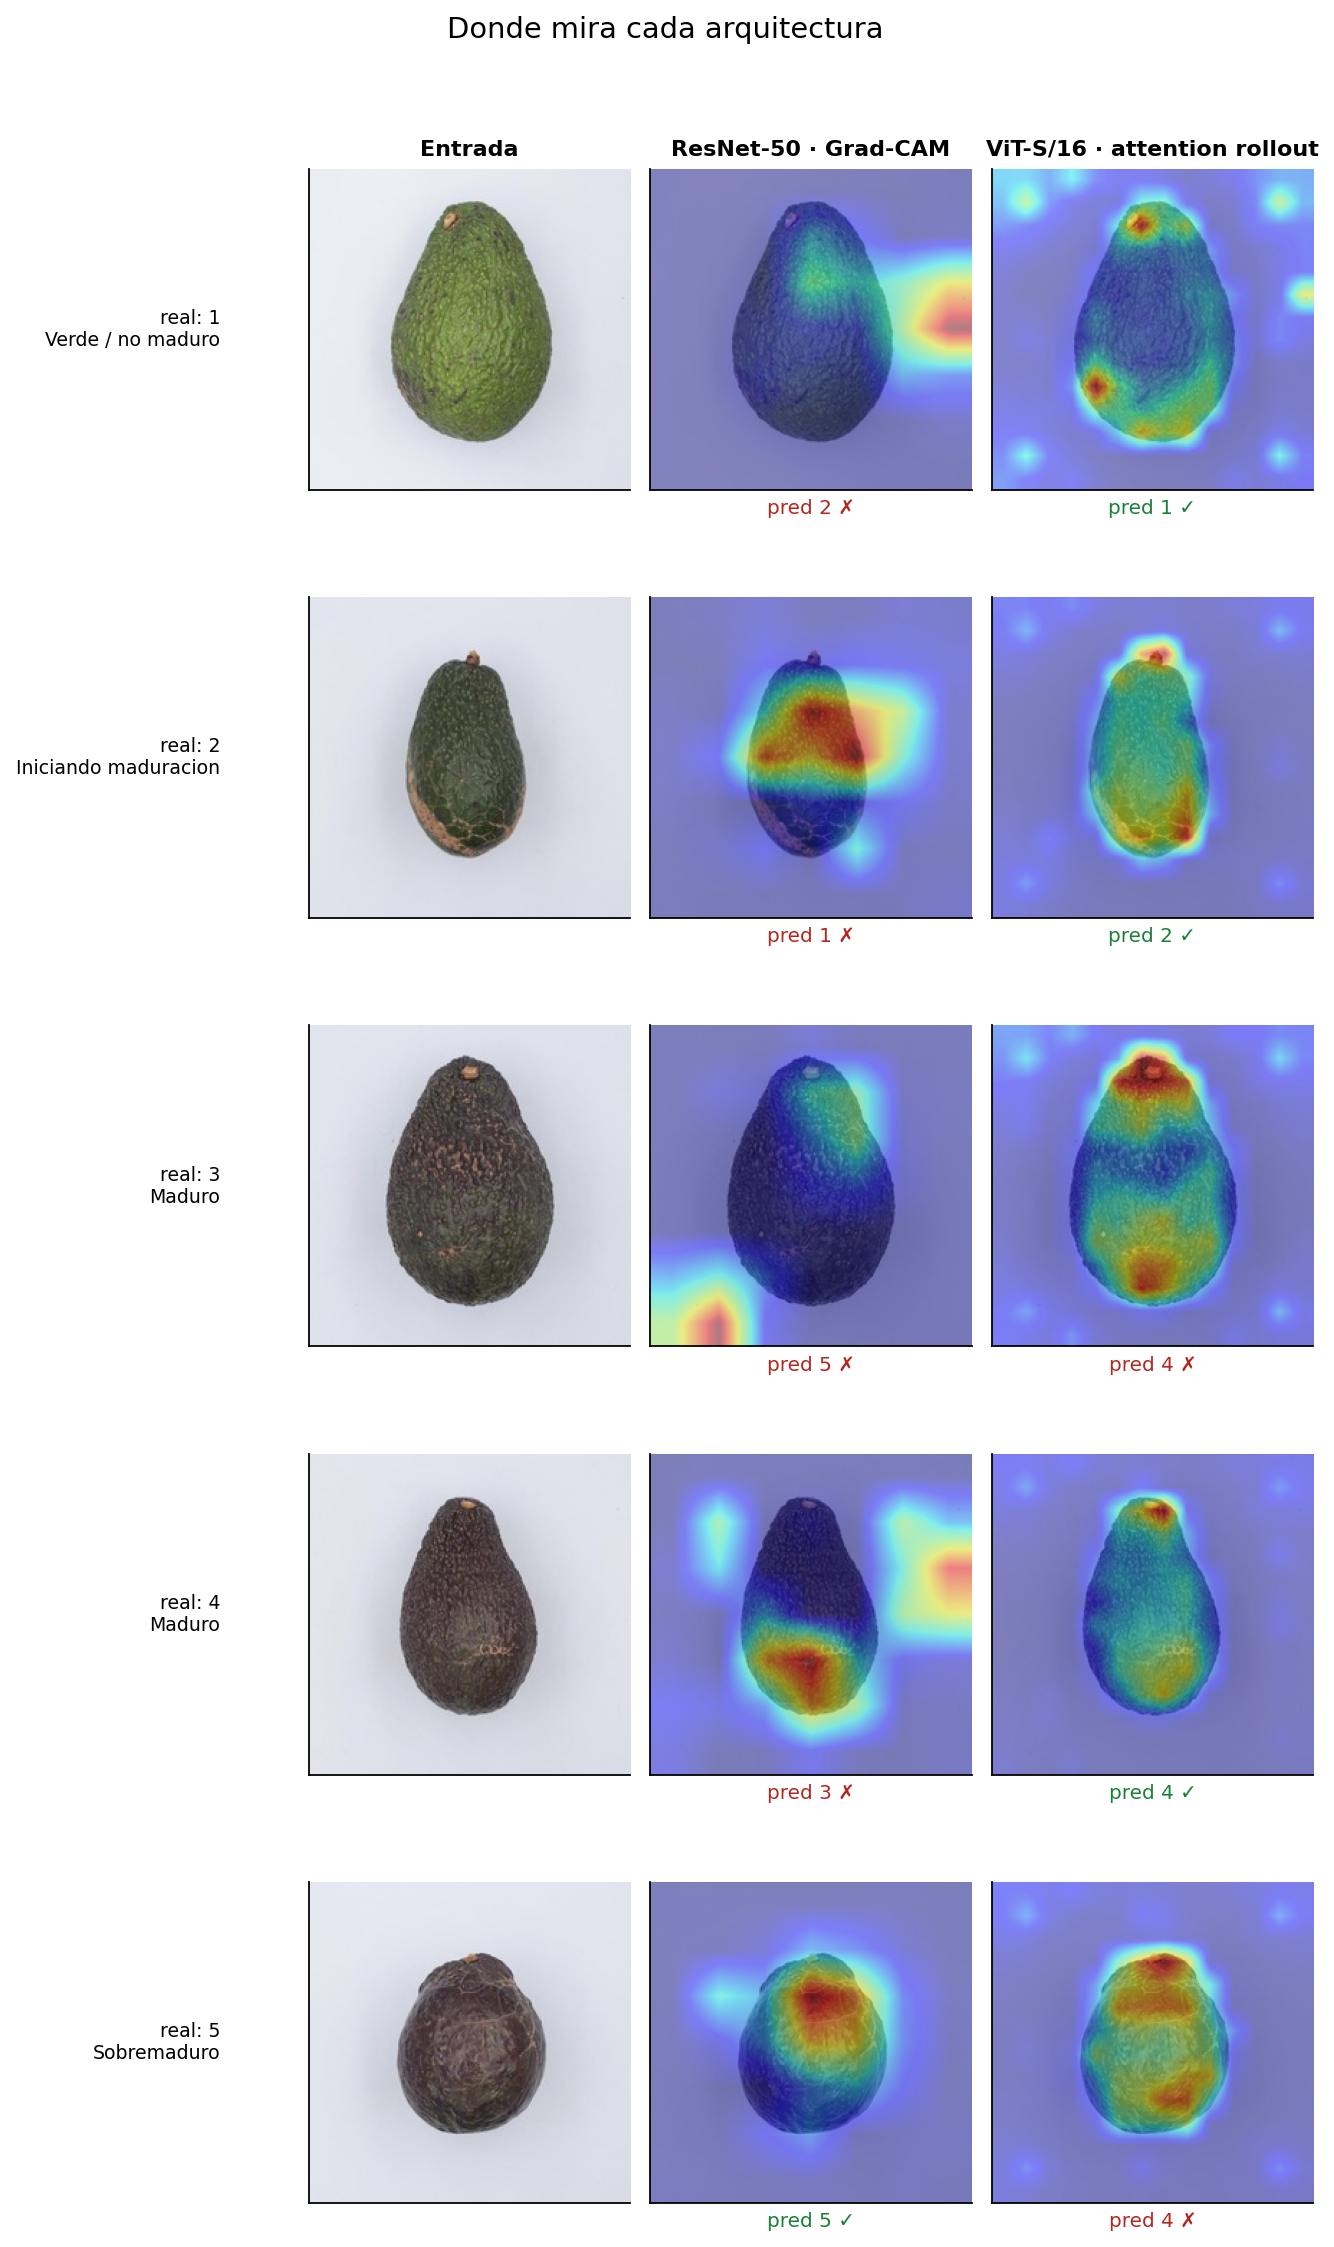
\includegraphics[width=\textwidth,height=5.4cm,keepaspectratio]{20-interpretabilidad-desacuerdo}
\end{center}
\end{column}
\begin{column}{0.66\textwidth}
{\tiny
\setlength{\itemsep}{0.25em}
\begin{itemize}
  \item Rojo = la zona que más influyó en la decisión; azul = la que casi no se usó.
  \item Cada red se abre con una técnica distinta, porque por dentro funcionan distinto. Las dos responden la misma pregunta.
  \item {\bfseries La ResNet se concentra en puntos chicos: una mancha, una arruga, una zona oscura.}
  \item {\bfseries El ViT reparte la mirada por áreas más grandes de la cáscara.}
  \item {\bfseries Un hallazgo incómodo y honesto:}
  \item En varios de los casos en que las dos redes discrepan, la ResNet está mirando el \emph{fondo}, fuera de la fruta. Y son justamente esos los casos en que se equivoca. Sin esta figura no lo habríamos notado.
\end{itemize}
}
\end{column}
\end{columns}
\end{frame}

\begin{frame}{\textquestiondown{}Cuál llevaríamos a una planta empacadora?}{No gana el más preciso: gana el que rinde mejor por lo que cuesta}
{\tiny
\centering
\begin{tabular}{l >{\centering\arraybackslash}p{0.15\textwidth} c >{\raggedright\arraybackslash}p{0.36\textwidth}}
\toprule
\rowcolor{verdeosc}\color{white}\bfseries Modelo & \color{white}\bfseries Acierta o se pasa por uno & \color{white}\bfseries Cuesta & \color{white}\bfseries Veredicto \\
\midrule
\rowcolor{verdecla!22}ResNet-50 & 99{,}2\,\% & 1{,}00$\times$ & La que recomendamos. Es la referencia. \\
ViT-S/16 & 99{,}5\,\% & 1{,}04$\times$ & Empata, cuesta lo mismo y se entrena en la mitad del tiempo. \\
Híbrido: fusión tardía & 99{,}5\,\% & 2{,}04$\times$ & Mejora poquito y cuesta el doble. No lo vale. \\
ViT-Hybrid R26+S/32 & 99{,}6\,\% & 0{,}84$\times$ & Mejor y más barato, pero estudió con más fotos: no es comparación limpia. \\
\bottomrule
\end{tabular}
}
\vspace{0.5em}
{\scriptsize
\setlength{\itemsep}{0.22em}
\begin{itemize}
  \item {\bfseries En una planta hay que clasificar miles de paltas por hora.}
  \item Probablemente en un computador común, sin tarjeta gráfica potente. Ahí el costo de cada foto importa tanto como el acierto.
  \item {\bfseries Si dos modelos empatan, gana el más barato.}
  \item Duplicar el costo para ganar unas décimas no se justifica.
  \item {\bfseries Y ya estamos en el techo de lo exigible.}
  \item Con más del 99\,\% de aciertos dentro de un escalón, lo que queda de error probablemente también lo cometería una persona.
\end{itemize}
}
\end{frame}

\begin{frame}{Demo}{Subir una foto y ver qué responde el modelo}
{\small
\setlength{\itemsep}{0.35em}
\begin{itemize}
  \item {\bfseries Se elige el modelo, se sube la foto y aparece la respuesta.}
  \item Muestra qué tan seguro está de cada uno de los 5 estados, y qué hacer con esa palta: dejarla madurar, venderla hoy o descartarla.
  \item {\bfseries Muestra también dónde miró para decidir.}
  \item No es una caja negra: se ve pintada sobre la foto la zona que usó.
  \item {\bfseries Avisa cuando no está seguro.}
  \item Si duda entre dos estados vecinos lo dice, en vez de responder con falsa confianza. Ahí conviene que mire una persona.
  \item {\bfseries Los ejemplos que trae cargados son paltas que ningún modelo vio nunca.}
  \item Y advierte en pantalla que fue entrenado con fotos de laboratorio.
\end{itemize}
}
\cierre{\texttt{python app/gradio\_app.py} $\rightarrow$ \texttt{http://localhost:7860}}
\end{frame}

\begin{frame}{Conclusiones y trabajo futuro}{Qué aprendimos y qué sigue}
{\scriptsize
\setlength{\itemsep}{0.28em}
\begin{itemize}
  \item {\bfseries Con el mismo tamaño y el mismo estudio previo, las dos redes resuelven esto igual de bien.}
  \item La pregunta interesante no era cuál gana, sino en qué se diferencian. Y la diferencia no está en el techo que alcanzan: está en cuántos datos necesitan para llegar.
  \item {\bfseries El límite de esta tarea lo pone quien etiquetó las fotos, no la red.}
  \item Como nadie revisó esas etiquetas dos veces, no sabemos cuánto del error que queda es del modelo y cuánto es desacuerdo entre humanos.
  \item {\bfseries Qué haríamos ahora, en orden de importancia:}
  \item 1) Salir a sacar fotos con celular en un packing chileno y medir cuánto cae. 2) Enseñarle explícitamente que las clases están ordenadas, cosa que hoy solo se le pide al evaluar. 3) Predecir directamente cuántos días de vida le quedan a la palta, que es lo que de verdad necesita la cadena de frío.
\end{itemize}
}
\cierre{\texttt{github.com/cmartinez1524/clasificacion-de-paltas}}
\end{frame}

{
\setbeamercolor{background canvas}{bg=grisFondo}
\begin{frame}[plain]
  \vfill
  \hspace{0.6cm}{\color{verdecla}\fontsize{54}{58}\selectfont\bfseries A}%
  \hspace{0.5cm}{\color{verdeosc}\Huge\bfseries Anexo}
  \vfill
\end{frame}
}

\begin{frame}{Anexo: todas las métricas}{Test: 2.262 imágenes de 72 frutas nunca vistas}
{\scriptsize
\centering
\begin{tabular}{lcccccccc}
\toprule
\rowcolor{verdeosc}\color{white}\bfseries Modelo & \color{white}\bfseries Params & \color{white}\bfseries GFLOPs & \color{white}\bfseries QWK & \color{white}\bfseries Accuracy & \color{white}\bfseries Macro-F1 & \color{white}\bfseries MAE & \color{white}\bfseries Acc. $\pm$1 & \color{white}\bfseries min \\
\midrule
ResNet-50 & 23{,}5\,M & 8{,}2 & 0{,}9356 & 74{,}6\,\% & 0{,}735 & 0{,}262 & 99{,}2\,\% & 10 \\
ViT-S/16 & 21{,}7\,M & 8{,}5 & 0{,}9313 & 72{,}2\,\% & 0{,}711 & 0{,}282 & 99{,}5\,\% & 5 \\
ResNet-50 (scratch) & 23{,}5\,M & 8{,}2 & 0{,}9152 & 67{,}2\,\% & 0{,}655 & 0{,}352 & 97{,}7\,\% & 18 \\
ViT-S/16 (scratch) & 21{,}7\,M & 8{,}5 & 0{,}8891 & 61{,}2\,\% & 0{,}579 & 0{,}409 & 98{,}1\,\% & 6 \\
Híbrido: fusión tardía & 46{,}4\,M & 16{,}7 & 0{,}9410 & 76{,}7\,\% & 0{,}760 & 0{,}238 & 99{,}5\,\% & 4 \\
ViT-Hybrid R26+S/32 & 36{,}0\,M & 6{,}9 & 0{,}9411 & 76{,}2\,\% & 0{,}752 & 0{,}242 & 99{,}6\,\% & 15 \\
\bottomrule
\end{tabular}
}
\vspace{0.5em}
{\tiny
\setlength{\itemsep}{0.18em}
\begin{itemize}
  \item \textbf{QWK}: kappa de Cohen con pesos cuadráticos. Penaliza el error según el cuadrado de la distancia entre clases y corrige por acuerdo azaroso. Es la métrica con la que elegimos el mejor modelo.
  \item \textbf{MAE}: error medio en escalones del índice de madurez.
  \item \textbf{Acc. $\pm$1}: fracción de predicciones en la clase correcta o una adyacente.
  \item \textbf{Macro-F1}: F1 promediado por clase; controla que las clases minoritarias no queden abandonadas.
\end{itemize}
}
\end{frame}

\begin{frame}{Anexo: pruebas estadísticas}{Diferencias contra ResNet-50, con intervalo de confianza del 95\,\%}
{\scriptsize
\setlength{\itemsep}{0.25em}
\begin{itemize}
  \item {\bfseries ViT-S/16: $\Delta$QWK $= $-$0{,}0042$, IC 95\,\% $[$-$0{,}0095, +0{,}0006]$, $p=0{,}095$ $\rightarrow$ \nosig}
  \item {\bfseries ResNet-50 (scratch): $\Delta$QWK $= $-$0{,}0203$, IC 95\,\% $[$-$0{,}0283, $-$0{,}0123]$, $p=0{,}000$ $\rightarrow$ \sig}
  \item {\bfseries ViT-S/16 (scratch): $\Delta$QWK $= $-$0{,}0465$, IC 95\,\% $[$-$0{,}0692, $-$0{,}0316]$, $p=0{,}000$ $\rightarrow$ \sig}
  \item {\bfseries Híbrido: fusión tardía: $\Delta$QWK $= +0{,}0055$, IC 95\,\% $[+0{,}0021, +0{,}0087]$, $p=0{,}001$ $\rightarrow$ \sig}
  \item {\bfseries ViT-Hybrid R26+S/32: $\Delta$QWK $= +0{,}0055$, IC 95\,\% $[+0{,}0005, +0{,}0104]$, $p=0{,}031$ $\rightarrow$ \sig}
  \item Los intervalos y los $p$-valores salen de un \emph{bootstrap pareado agrupado por fruta}: las 2.262 imágenes vienen de solo 72 paltas, así que remuestrear imágenes daría intervalos artificialmente angostos. Se remuestrean frutas, 2.000 réplicas.
\end{itemize}
}
\end{frame}

\begin{frame}{Anexo: desglose por temperatura de almacenamiento}{Sirve para detectar si el modelo se apoya en un atajo}
{\tiny
\centering
\begin{tabular}{llccc}
\toprule
\rowcolor{verdeosc}\color{white}\bfseries Modelo & \color{white}\bfseries Grupo & \color{white}\bfseries n & \color{white}\bfseries Accuracy & \color{white}\bfseries MAE \\
\midrule
ResNet-50 & T10 (10\,\textdegree C) & 1350 & 75{,}3\,\% & 0{,}259 \\
ResNet-50 & T20 (20\,\textdegree C) & 466 & 75{,}1\,\% & 0{,}249 \\
ResNet-50 & Tamb & 446 & 71{,}8\,\% & 0{,}285 \\
ViT-S/16 & T10 (10\,\textdegree C) & 1350 & 73{,}9\,\% & 0{,}267 \\
ViT-S/16 & T20 (20\,\textdegree C) & 466 & 68{,}7\,\% & 0{,}318 \\
ViT-S/16 & Tamb & 446 & 71{,}1\,\% & 0{,}291 \\
Híbrido: fusión tardía & T10 (10\,\textdegree C) & 1350 & 77{,}7\,\% & 0{,}231 \\
Híbrido: fusión tardía & T20 (20\,\textdegree C) & 466 & 76{,}2\,\% & 0{,}240 \\
Híbrido: fusión tardía & Tamb & 446 & 74{,}4\,\% & 0{,}256 \\
ViT-Hybrid R26+S/32 & T10 (10\,\textdegree C) & 1350 & 77{,}7\,\% & 0{,}227 \\
ViT-Hybrid R26+S/32 & T20 (20\,\textdegree C) & 466 & 75{,}8\,\% & 0{,}247 \\
ViT-Hybrid R26+S/32 & Tamb & 446 & 72{,}0\,\% & 0{,}280 \\
\bottomrule
\end{tabular}
}
\cierre{Desempeño parejo entre grupos: el modelo no está usando el atajo \guillemotleft{}verde $\Rightarrow$ refrigerada\guillemotright{}.}
\end{frame}

\end{document}
